%************************************************
\chapter{DeepGamma: A deep learning model for activity coefficient prediction}\label{ch:deep_gamma} 
%************************************************

\section{Introduction}

Vapor-liquid equilibrium thermodynamics play an essential role in a wide variety of fields in the basic and applied sciences. For example, chemical reactions often happen in between the vapor and liquid phase, where vapor produced by a reaction is extracted to drive conversion or a reactant is introduced as a vapor. Similarly, large scale chemical processes require separation of mixtures into components to purify a valuable product. One ubiquitous method for achieving such separations is distillation, which relies on differences in boiling points of mixtures to achieve separation.

In order to design and engineer systems which contain vapor-liquid equilibrium, thermodynamic equations are utilized. Thermodynamic equations describe the relationship between the composition of the liquid and the vapor at a given temperature and pressure. One well-known thermodynamic equation is Raoult's Law: 

\begin{equation}
    \label{ideal-gas}
    y_i P = x_iP_i^{sat}(T)
\end{equation}

where $y_i$ and $x_i$ are the vapor and liquid compositions of component $i$ of the mixture respectively, $P$ is the absolute pressure, and $P_i^{sat}(T)$ is the vapor pressure at temperature $T$. Raoult's law describes non-interacting ideal systems, yet it fails to properly predict vapor-liquid equilibrium the wide variety of mixtures used in industrial chemical processes. Therefore, the simplified gamma-phi equation was developed to describe deviations from ideality:

\begin{equation}
    \label{gamma-phi}
    y_i P = x_i \gamma_i(x,T,P)   \exp \biggl(\frac{V_i^L(P-P_i^{sat}(T))}{RT}\biggr)
\end{equation}

where $\gamma_i(\mathbf x,T,P)$ is the activity coefficient at liquid composition $\mathbf x$,  temperature $T$, and pressure $P$; $V_i^L$ is the specific volume and $P_i^{sat}$ is the vapor pressure.  

Activity coefficients are the unknown parameters in the gamma-phi thermodynamic equation that correct for deviations from ideality. These activity coefficients must be predicted for each new mixture using thermodynamic models such as the non-random two liquid model \cite{Renon1968}. 

Unfortunately, the vapor-liquid equilibrium experiments required to parameterize thermodynamic models for predicting activity coefficients are notoriously time-intensive to complete. Classical thermodynamic measurement apparatus such as stills require equilibrium to be reached at each temperature and pressure combination before a measurement is taken \cite{Ronc1976, Dechambre2014}. This equilibration process can take anywhere from minutes to hours, meaning a full set of experiments for a new mixture can take weeks to months. As a result, vapor liquid equilibrium experiments are executed very selectively.

To reduce the time required for parameterizing thermodynamic models for predicting activity coefficients, there is a large body of research focused on directly predicting the parameters from molecular structures. This work ranges from simple counting of functional groups \cite{Fredenslund1975} to density functional theory \cite{ Klamt2010} and machine learning \cite{Urata2002, Nami2011,  Jirasek2020}.  However, these prediction approaches often only cover a small subset of all mixture types (e.g., only hydrocarbons) or require significant calculation times. Thus, there is a need for a general, fast and accurate method for predicting activity coefficients \textit{a priori}.

Herein, we introduce \textit{DeepGamma}, a deep learning model for fast predictions of activity coefficients directly from molecular structures.  We leverage  message passing neural networks (MPNN) to reproduce the results of quantum simulations for predicting activity coefficients without computational expense. Specifically, our model decreases the time required for calculations by a factor of 1900. Our work focuses on predicting activity coefficients of binary mixtures as a first proof of concept. 

\section{Background}

We classify existing methods for predicting activity coefficients into three categories: group-contribution methods, quantum chemistry based methods and machine learning methods. 

\subsubsection{Group Contribution Methods}

Group contribution methods such as UNIFAC were originally developed in the 1970s and predict the activity coefficient as a weighted sum of the occurrence of a predetermined set of basis functions with inputs as the chemical functional groups in each component \cite{Fredenslund1975}. UNIFAC specifically predicts the natural logarithm of the activity coefficient of component $i$ in  a mixture as the sum of a combinatorial term $\ln \gamma_i^C$ and a residual term $\ln \gamma_i^R$:

\begin{equation}
    \ln \gamma_i = \ln \gamma_i^C + \ln \gamma_i^R
\end{equation}

The combinatorial term represents the combination of different functional groups:

\begin{equation}
    \ln  \gamma^C_i = \ln \frac{\Phi_i}{x_i} + \frac{z}{2} q_i \ln \frac{\theta_i}{\Phi_i} + l_i - \frac{\Phi_i}{x_i} \sum_jx_jl_j
\end{equation}

where $\Phi_i$ and $\theta_i$ are the weighted molar segment area and area for component. These variables in addition to $l_j$ are a function of $r_i$, $z$ and $q_i$, which are  in turn functions of the group volume and surface area parameters $R_k$ and $Q_k$ for tabulated functional groups:

\begin{equation}
    \Phi_i  = \frac{r_i x_i}{\sum_j r_j x_j}
\end{equation}

\begin{equation}
    \theta_i = \frac{q_i x_i}{\sum_j q_j x_j}
\end{equation}

\begin{equation}
    l_i = \frac{z}{2}(r_i-q_i) - (r_i -1) \;\; z=10
\end{equation}

\begin{equation}
    r_i  = \sum_k = v_k^i R_k
\end{equation}

\begin{equation}
    q_i = \sum_k v_k^i Q_k
\end{equation}

$v_k^i$ is the number of groups of type $k$ in component $i$.

The residual term represents inter-group interactions. It is composed of the group residual activity coefficient $\Gamma_k$ and  $\Gamma_k^{(i)}$, the residual activity coefficient of group k in reference solution with only component $i$.

\begin{equation}
    \ln \gamma^R_i = \sum_k v_k^{(i)}(\ln \Gamma_k - \ln \Gamma_k^{(i)})
\end{equation}

\begin{equation}
    \ln \Gamma_k = Q_k \biggl[1 - \ln \bigl(\sum_m \theta_m \psi_{mk}\bigr) - \sum_m \frac{\theta_m \Psi_{km}}{\sum_n \theta_n \Psi_{nm}} \biggr]
\end{equation}

\begin{equation}
    \theta_m = \frac{Q_m X_m}{\sum_n Q_n X_n}
\end{equation}

\begin{equation}
    \Psi_{mn} = \exp{\frac{a_{mn}}{T}}
\end{equation}

where $a_{mn}$ is a binary interaction parameter. 

While UNIFAC provides fast predictions, the accuracy of the model is limited by the interactions explicitly accounted for in each basis function. It can be challenging to hand-craft all such interactions as they can often extend between several atoms.

\subsubsection{Quantum Chemistry}

The second set of methods are quantum chemistry methods. These simulations often use a combination of molecular dynamics and density functional theory (DFT) calculations to predict activity coefficients for each mixture component \cite{Constantinescu2005}. COSMO-RS is one of the most reliable computational methods for liquid-phase thermodynamic predictions \cite{Klamt1995, Klamt2010}. It relies on the theory of screening charges, which states that every element of a surface of a dissolved solute must be complemented by an opposite charge in the solvent. The charge surface around a solute is divided into infinitesimally small pieces, which are then integrated to find the charge density. This charge density can then be used to calculate activity coefficients. The charge density is calculated via rigorous DFT calculations or a much faster quantitative structure-property relationship based on a database of over 65,000 pre-calculated compounds. COSMO-RS and a related method named COSMO-SAC have been applied in calculations of VLE \cite{Constantinescu2005}, liquid-liquid equilibrium (LLE) \cite{Dechambre2014} and vapor-liquid-liquid-equilibrium (VLLE) curves \cite{Kundu2011}.

The downside of COSMO methods is that they are often not accurate for polar compounds \cite{Constantinescu2005, Kundu2011}. This is often due to the lack of theory for the hydrogen bonding present in these systems \cite{Kundu2011}. Another challenging aspect of COSMO-RS is the computational intensity of DFT calculations for new mixtures, though this can be somewhat alleviated by a less accurate method for predictions of charge surfaces from molecular structures \cite{Loschen2012}. 

\subsubsection{Machine Learning}

There has been significant work on directly predicting infinite dilution activity coefficients from molecular structures and closely related free solvation energies using simple neural networks\cite{Urata2002, RamirezBeltran2009, Nami2011, Behrooz2017}, matrix completion\cite{Jirasek2020} and  graph neural networks \cite{Vermeire2021, Felton2022, SanchezMedina2022, Qin2022, Rittig2022}. However, the limitation of these works is their lack of thermodynamic consistency and other guarantees that come with rigorously derived equations of state. To overcome this problem, recent work has attempted to predict EoS parameters \cite{Abbasi2020, Madani2021, Abdallahelhadj2022, Winter2022}, which can be in turn used to predict thermodynamic outcomes.

After the publication of \textit{DeepGamma}, Winter et al developed a model for predicting activity coefficients using transformer models. Specifically, they predict the parameters of the NRTL model, for any mixture \cite{Winter2022}. By doing so, they achieve three benefits thermodynamic consistency and easy application in existing process simulation software. However, the NRTL model is known to have highly correlated parameters which lead to a wide range of parameterizations for a particular mixture. 

Additionally, I note that Habicht et al. recently developed a feed forward neural network model to predict PC-SAFT parameters \cite{Habicht2023}.  Their model architecture differs from ours, and they predict PC-SAFT parameters, while our method includes the polar and associating terms (PCP-SAFT). 


\section{Methods}
\subsection{Models}

\noindent
\textbf{Message passing neural networks:} Molecules can be treated as graphs with atoms as nodes and bonds as edges. Therefore, message passing neural networks (MPNN) that operate on graphs can be used for end-to-end prediction of molecular properties \cite{Gilmer2017}.  In a MPNN, each node passes a vector (i.e., its current features) to its neighbor. This  vector is called a message. In each layer, a permutation invariant aggregation function such as the mean is used to calculate the total message for each node prior to passing through an activation function to get a new value for each node.  In contrast to traditional fixed fingerprints like ECFP \cite{Rogers2010}, the best feature vector is learned end-to-end for each property prediction task.

One type on MPNN is a directed message passing neural network (D-MPNN) in which the encoder acts on edges (bonds) instead of nodes (atoms) to improve stability of training \cite{Yang2019}. Yang, Swanson and colleagues showed D-MPNNs have superior performance to other tools such as gradient boosted trees for property prediction tasks \cite{Yang2019}. Formally, a molecule in a D-MPNN is considered to be a graph $G$ with edges $e_{vw}$ and nodes $v$ and $w$ with atom features $x_v$. A message passing update $m_v^{t}$ is as follows:

\begin{equation}
    m_v^{t+1} = \sum_{w\in N(v)} M_t(h_v^t, h_w^t, e_{vw})
\end{equation}

\begin{equation}
    h_v^{t+1} = U_t(h_v^t, m_v^{t+1})
\end{equation}

where $M_t$ is the message function, $U_t$ is the update function and $h_v^{t}$ is the hidden state at step $t$. To obtain predictions $\hat y$, the outputs of the last message passing step $T$ are passed through a feed forward network $R$ in a readout phase:
 
\begin{equation}
    \hat y = R(h_v^T \in G)
\end{equation}

In addition to using outputs of the message passing steps as input to the feed forward network, additional features $f$ can also be added:

\begin{equation}
    \hat y = R(h_v^T \in G, f)
\end{equation}

In our case of predicting activity coefficients of binary mixtures at atmospheric pressure, we treat the temperature and composition as additional features. Therefore, the feed forward network can be written as:

\begin{equation}
   \ln \gamma(x,T)= R(h_v^T \in G, x, T)
\end{equation}

Note that we predict the natural logarithm of the activity coefficient since these values can vary over an order of magnitude.

We also explore the use of an architecture that uses 3D information in addition to 2D information. In particular, we use PaiNN, a model that use a an equivariant message passing that works with both rank 1 and 3 tensors. By doing so, the model improved predictions on vector properties such as the Dipole moment.

\noindent
\textbf{DeepGamma Polynomial:} Often, adding chemical knowledge into machine learning models can make them more accurate. In the case of activity coefficient prediction, it would be best to fit a thermodynamically consistent model such as the the non-random two liquid model (NRTL) \cite{Renon1968}. However, we found that many of the mixtures in our training set (see "Datasets") were difficult to fit using NRTL, often because the large correlations between its parameters \cite{Holler2019}. As shown in Figure \ref{fig:mnae_distribution}, the NRTL model had significant errors (>0.2) for many mixtures.

\begin{figure}
    \centering
    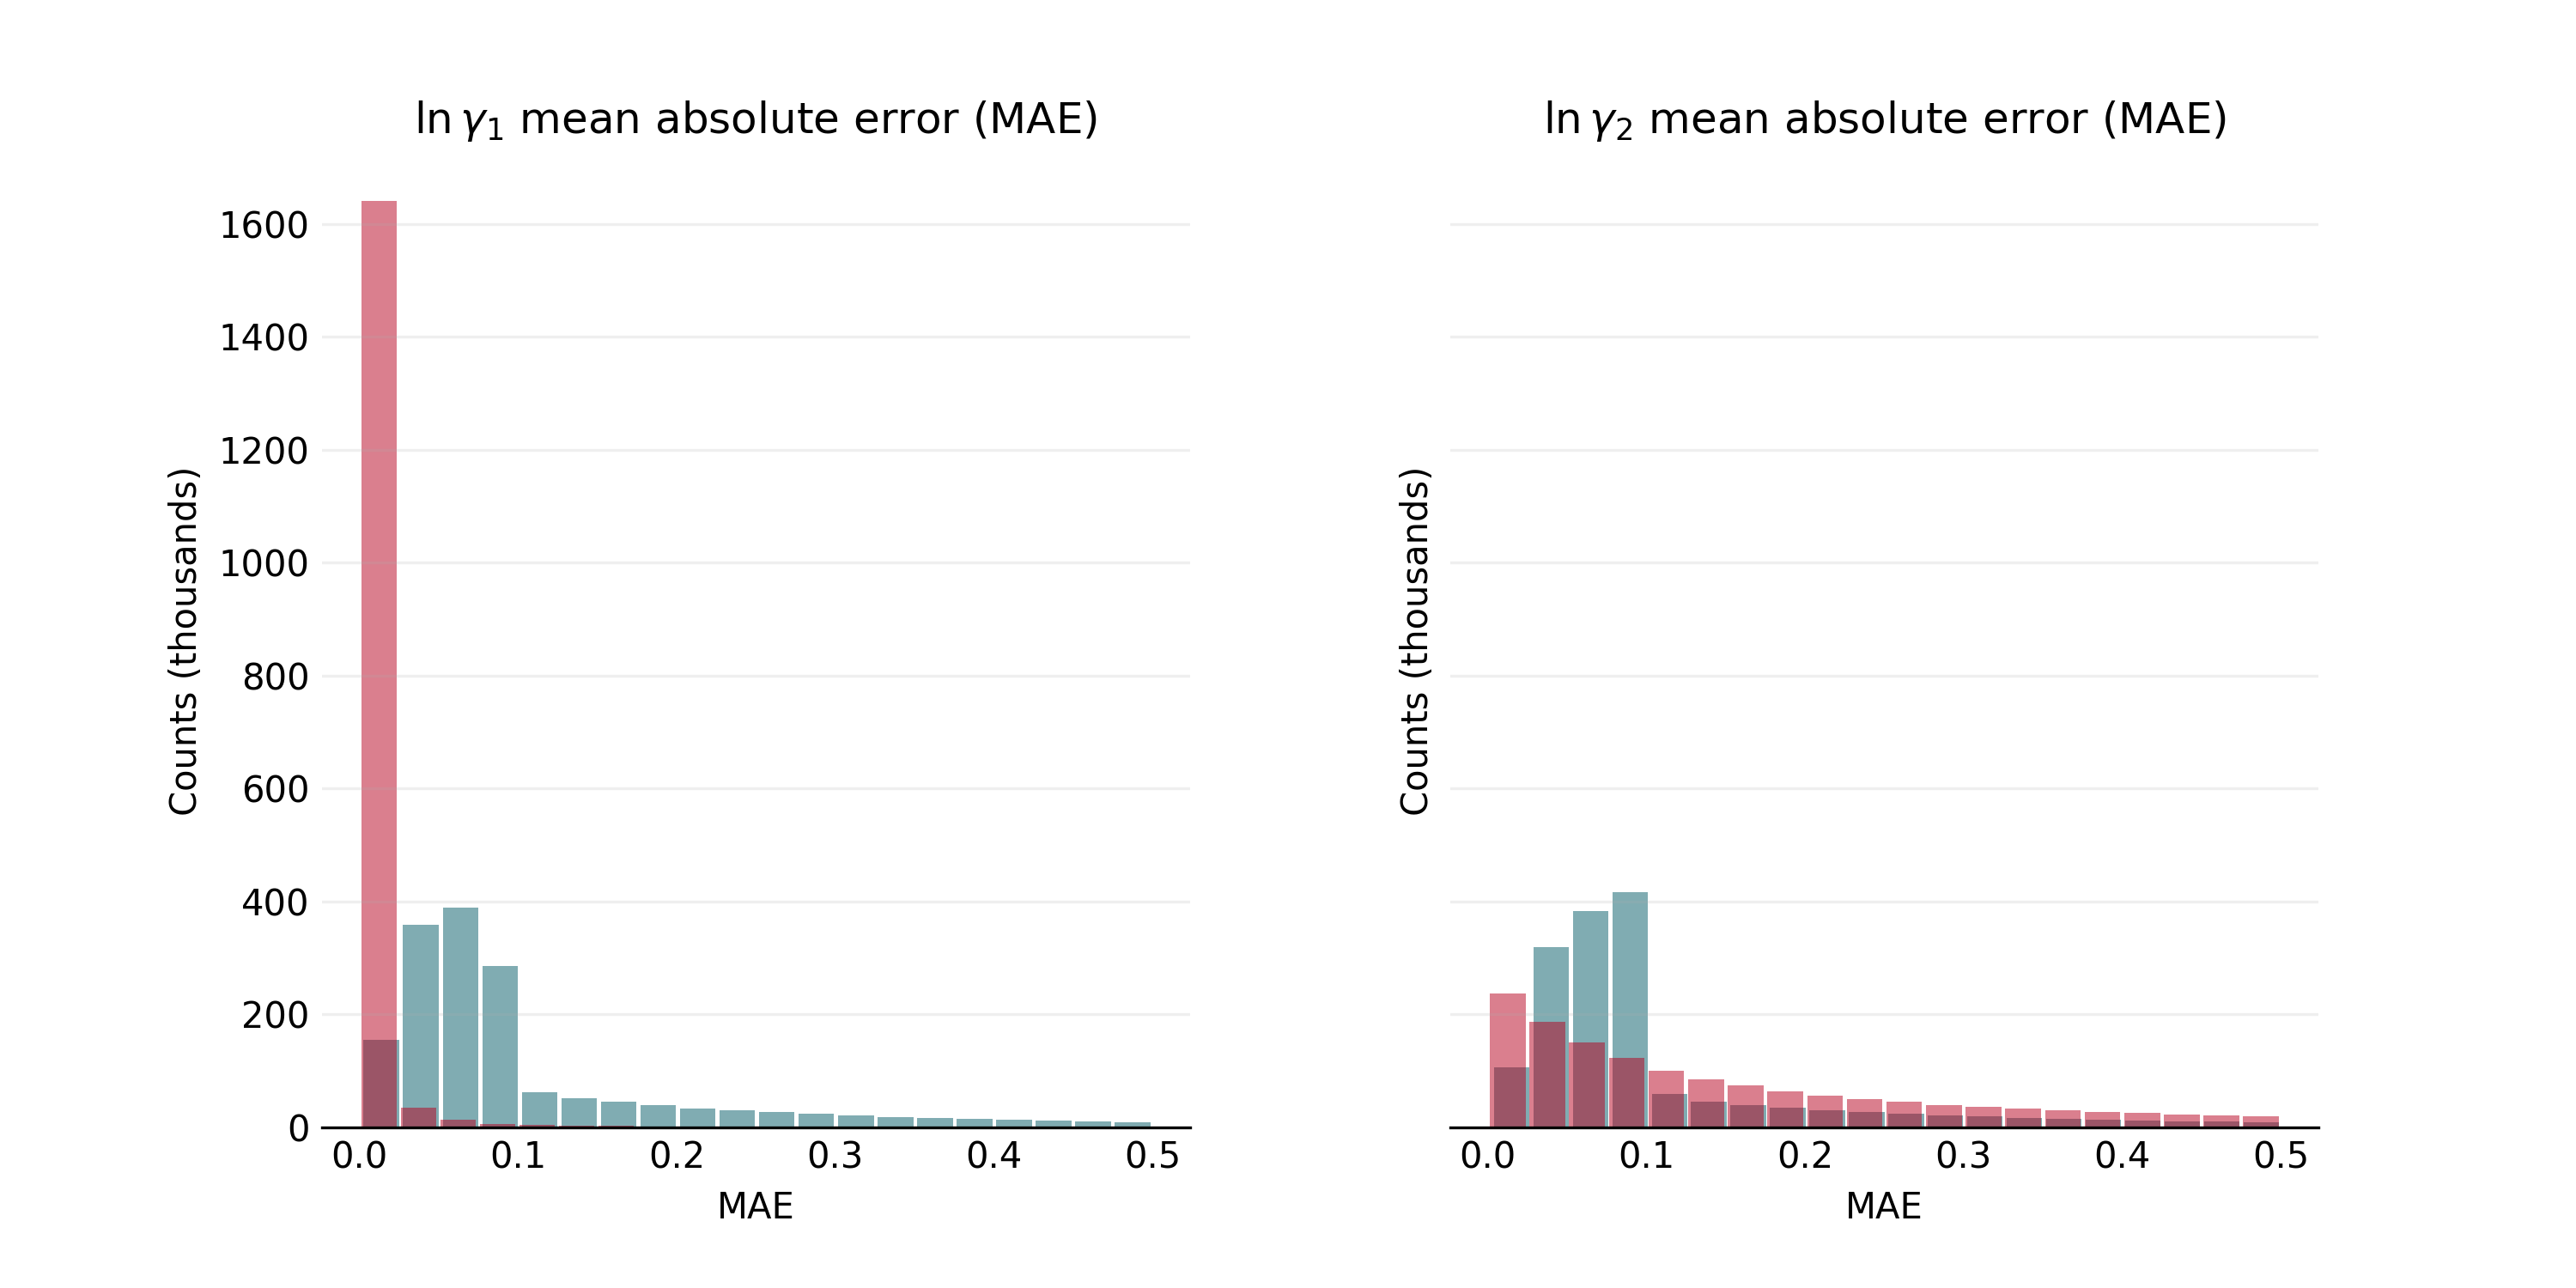
\includegraphics[width=\textwidth]{gfx/Chapter06/error_distribution_fitting_cosmo.png}
    \caption{Error distribution of mean normalized error of data fit using NRTL and polynomial models.}
    \label{fig:mnae_distribution}
\end{figure}

We found empirically that the activity coefficient curves fit well to a fourth order polynomial model. While this  polynomial form does not necessarily ensure Gibbs-Duheim thermodynamic consistency\footnote{The Gibbs-Duheim equation relates changes in chemical potential to changes in temperature and pressure. $\sum_{i=1}^I N_i d\mu_i$ = -SdT + VdP. At equilibrium, the right hand side becomes zero, so traditional thermodynamic models like NRTL obey the equation $\sum_{i=1}^I N_i d\mu_i=0$}, it should work well for the sole purpose of vapor liquid equilibrium activity coefficients (not liquid-liquid equilibrium for example). Therefore, we fitted fourth order polynomials to the activity coefficient data and used the D-MPNN to predict the coefficients of the polynomial model:

\begin{equation}
    \ln \gamma_i(x_i,T) = \sum_{j=0}^4 c_{ij}(T)x^j
\end{equation}

\begin{equation}
     \mathbf{c_{ij}} = R(h_v^T \in G, \mathbf{x}, T)
\end{equation}

In our results we compare direct prediction of activity coefficients and predicting polynomial coefficients.

\subsection{Datasets}

Previous work has demonstrated the power of transfer learning for improving predictions of D-MPNNs \cite{Vermeire2021}. We aim to obtain similar results for activity coefficient prediction, relying on two datasets.

\noindent
\textbf{Combisolv Solvation Energy Dataset:} Solvation energies describe the change in free energy when a gas molecule of a solute is placed into a solvent. Solvation energies are closely related to activity coefficients at infinite dilution \cite{Moine2017}, so encoder representations learned on this task could be useful for the downstream task of activity coefficient prediction. We utilize the Combisolv dataset, which contains the largest number of solvation energies publicly available to date: one million binary pairs of molecules calculated using COSMO-RS \cite{Vermeire2021}.

\noindent
\textbf{COSMO-RS Activity Coefficient Dataset:} We executed DFT calculations for over 18 million activity coefficients by taking all the binary pairs of 460 common solvent molecules from a previously published dataset \cite{Amar2019}. The activity coefficients were calculated in 5K temperature increments between the normal boiling points of the each binary pair, and 0.1 mol/mol composition grid was used. All activity coefficients were calculated at atmospheric pressure. COSMOtherm 2020 at the TZVPD fine fidelity level was utilized, and parameters were taken the 2020 COSMObase database \cite{Klamt2010}. These calculations took 41 days on a 24 core machine. 

\noindent
\textbf{Aspen Activity Coefficient Dataset:} The third set of data were obtained using the process modeling software, Aspen Plus. This was chosen due to the fact that the thermodynamic data used to simulate processes were obtained from the Dortmund Data Bank (DDB). A total of 2500 components were added to Aspen, from which temperature dependent non-random two liquid model binary parameters of binary VLE systems were retrieved via regression of literature data from Aspen’s VLE-IG databank. VLE systems were retrieved, from which the activity coefficients were calculated at mole fractions of zero to one in increments of 0.1 and 11K temperature increments. 



\section{Results}

\begin{table*}[t]
\centering
\caption{Validation and test mean absolute error of DeepGamma (DG) models on the COSMO-RS Activity  Coefficient Dataset. Best results are bolded. TLCB stands for transfer learning, where the encoder from the model trained on the Combisolv dataset is frozen and only the feedforward network is tuned. DGP stands for models which predict polynomial coefficients instead of activity coefficients directly. Time is training time in hours.}
% \renewcommand{\arraystretch}{1.2}
\label{cosmo_rs_results}
\begin{tabular}{lccllllllllll}
& & \multicolumn{2}{c}{Valid CONT} &  \multicolumn{2}{c}{Valid  INDP}  &  \multicolumn{2}{c}{Valid MIX}  &\multicolumn{2}{c}{Test MIX} &  \multicolumn{2}{c}{Test  INDP} \\
& Training (h) & $\ln\gamma_1$ & $\ln\gamma_2$ & $\ln\gamma_1$ & $\ln\gamma_2$ & $\ln\gamma_1$ & $\ln\gamma_2$ & $\ln\gamma_1$ & $\ln\gamma_2$ & $\ln\gamma_1$ & $\ln\gamma_2$ \\
\hline 
\textbf{DG}  &     62           & \textbf{0.02 }                               & \textbf{0.02  }                              & \textbf{0.07}                                & \textbf{0.07}                                & \textbf{0.07 }                               & \textbf{0.07  }                              &\textbf{ 0.06  }                              & \textbf{0.06  }                              & \textbf{0.06   }                             & \textbf{0.05 }                               \\
DG-TLCB &  36    & 0.04                                & 0.04                                & 0.09                                & 0.09                                & 0.08                                & 0.08                                & 0.07                                & 0.07                                & 0.07                                & 0.07                                \\
DGP &    6.2      & 0.10                                & 0.29                                & 0.16                                & 0.36                                & 0.14                                & 0.33                                & 0.14                                & 0.28                                & 0.13                                & 0.28                                \\
DGP-TLCB & 3.5 & 0.10                                & 0.29                                & 0.16                                & 0.36                                & 0.14                                & 0.33                                & 0.14                                & 0.28                                & 0.13                                & 0.28                               
\end{tabular}
\end{table*}

\textit{DeepGamma} is rapidly trained to reproduce results of COSMO-RS for activity coefficient prediction. It takes 2.5 days to train our best performing model, and predictions on more than 1M activity coefficients takes less than 30 minutes on a modern GPU. This is significant because generating the original data required over one month, representing a 1900x speed up.

% In all our tables, we report mean absolute error for each model and holdout set. We also report the time required for training, as this varies significantly between the full and pretrained models. Fitting the polynomial model required approximately 24 hours.

Results of training on the COSMO-RS activity coefficient dataset are shown in Table \ref{cosmo_rs_results}, the base DeepGamma model achieves the lowest mean absolute error on all holdout sets. Similar mean absolute errors are achieved on the validation and test datasets for all models. As expected, the Valid CONT holdout set has the lowest MAE due to the same molecules being in the training set and holdout set.  For the best performing base model, the INDP and MIX datasets have similar error profiles, indication that model has learned a good encoder representation.  Transfer learning models have slightly worse performance than the base models, but the transfer learning models take ~50\% less time to train. Part of the reason for poorer performance is that the Combisolv model was trained with a depth of four (i.e., number of message passing steps), while the COSMO-RS model only utilized three. Since each message passing step can cause changes in the atom representation, this difference in depth could effect quality of the final fingerprint formed. Interestingly, the DeepGamma Polynomial models have the worst performance of all models. Furthermore, there are significant differences in error between the different activity coefficients predicted by the DeepGamma Polynomial.  It is possible that further hyperparameter tuning could improve the accuracy of the model, particularly through changes in the encoder and feedforward network hidden size \cite{Yang2019, Vermeire2021}.

Results of training on the COSMO-RS activity coefficient dataset are shown in Table \ref{cosmo_rs_results}, the base DeepGamma model achieves the lowest mean absolute error on all holdout sets. Similar mean absolute errors are achieved on the validation and test datasets for all models. As expected, the Valid CONT holdout set has the lowest MAE due to the same molecules being in the training set and holdout set.  For the best performing base model, the INDP and MIX datasets have similar error profiles, indication that model has learned a good encoder representation.  Transfer learning models have slightly worse performance than the base models, but the transfer learning models take ~50\% less time to train. Part of the reason for poorer performance is that the Combisolv model was trained with a depth of four (i.e., number of message passing steps), while the COSMO-RS model only utilized three. Since each message passing step can cause changes in the atom representation, this difference in depth could effect quality of the final fingerprint formed. Interestingly, the DeepGamma Polynomial models have the worst performance of all models. Furthermore, there are significant differences in error between the different activity coefficients predicted by the DeepGamma Polynomial.  It is possible that further hyperparameter tuning could improve the accuracy of the model, particularly through changes in the encoder and feedforward network hidden size \cite{Yang2019, Vermeire2021}.

\begin{figure}[t]
    \centering
    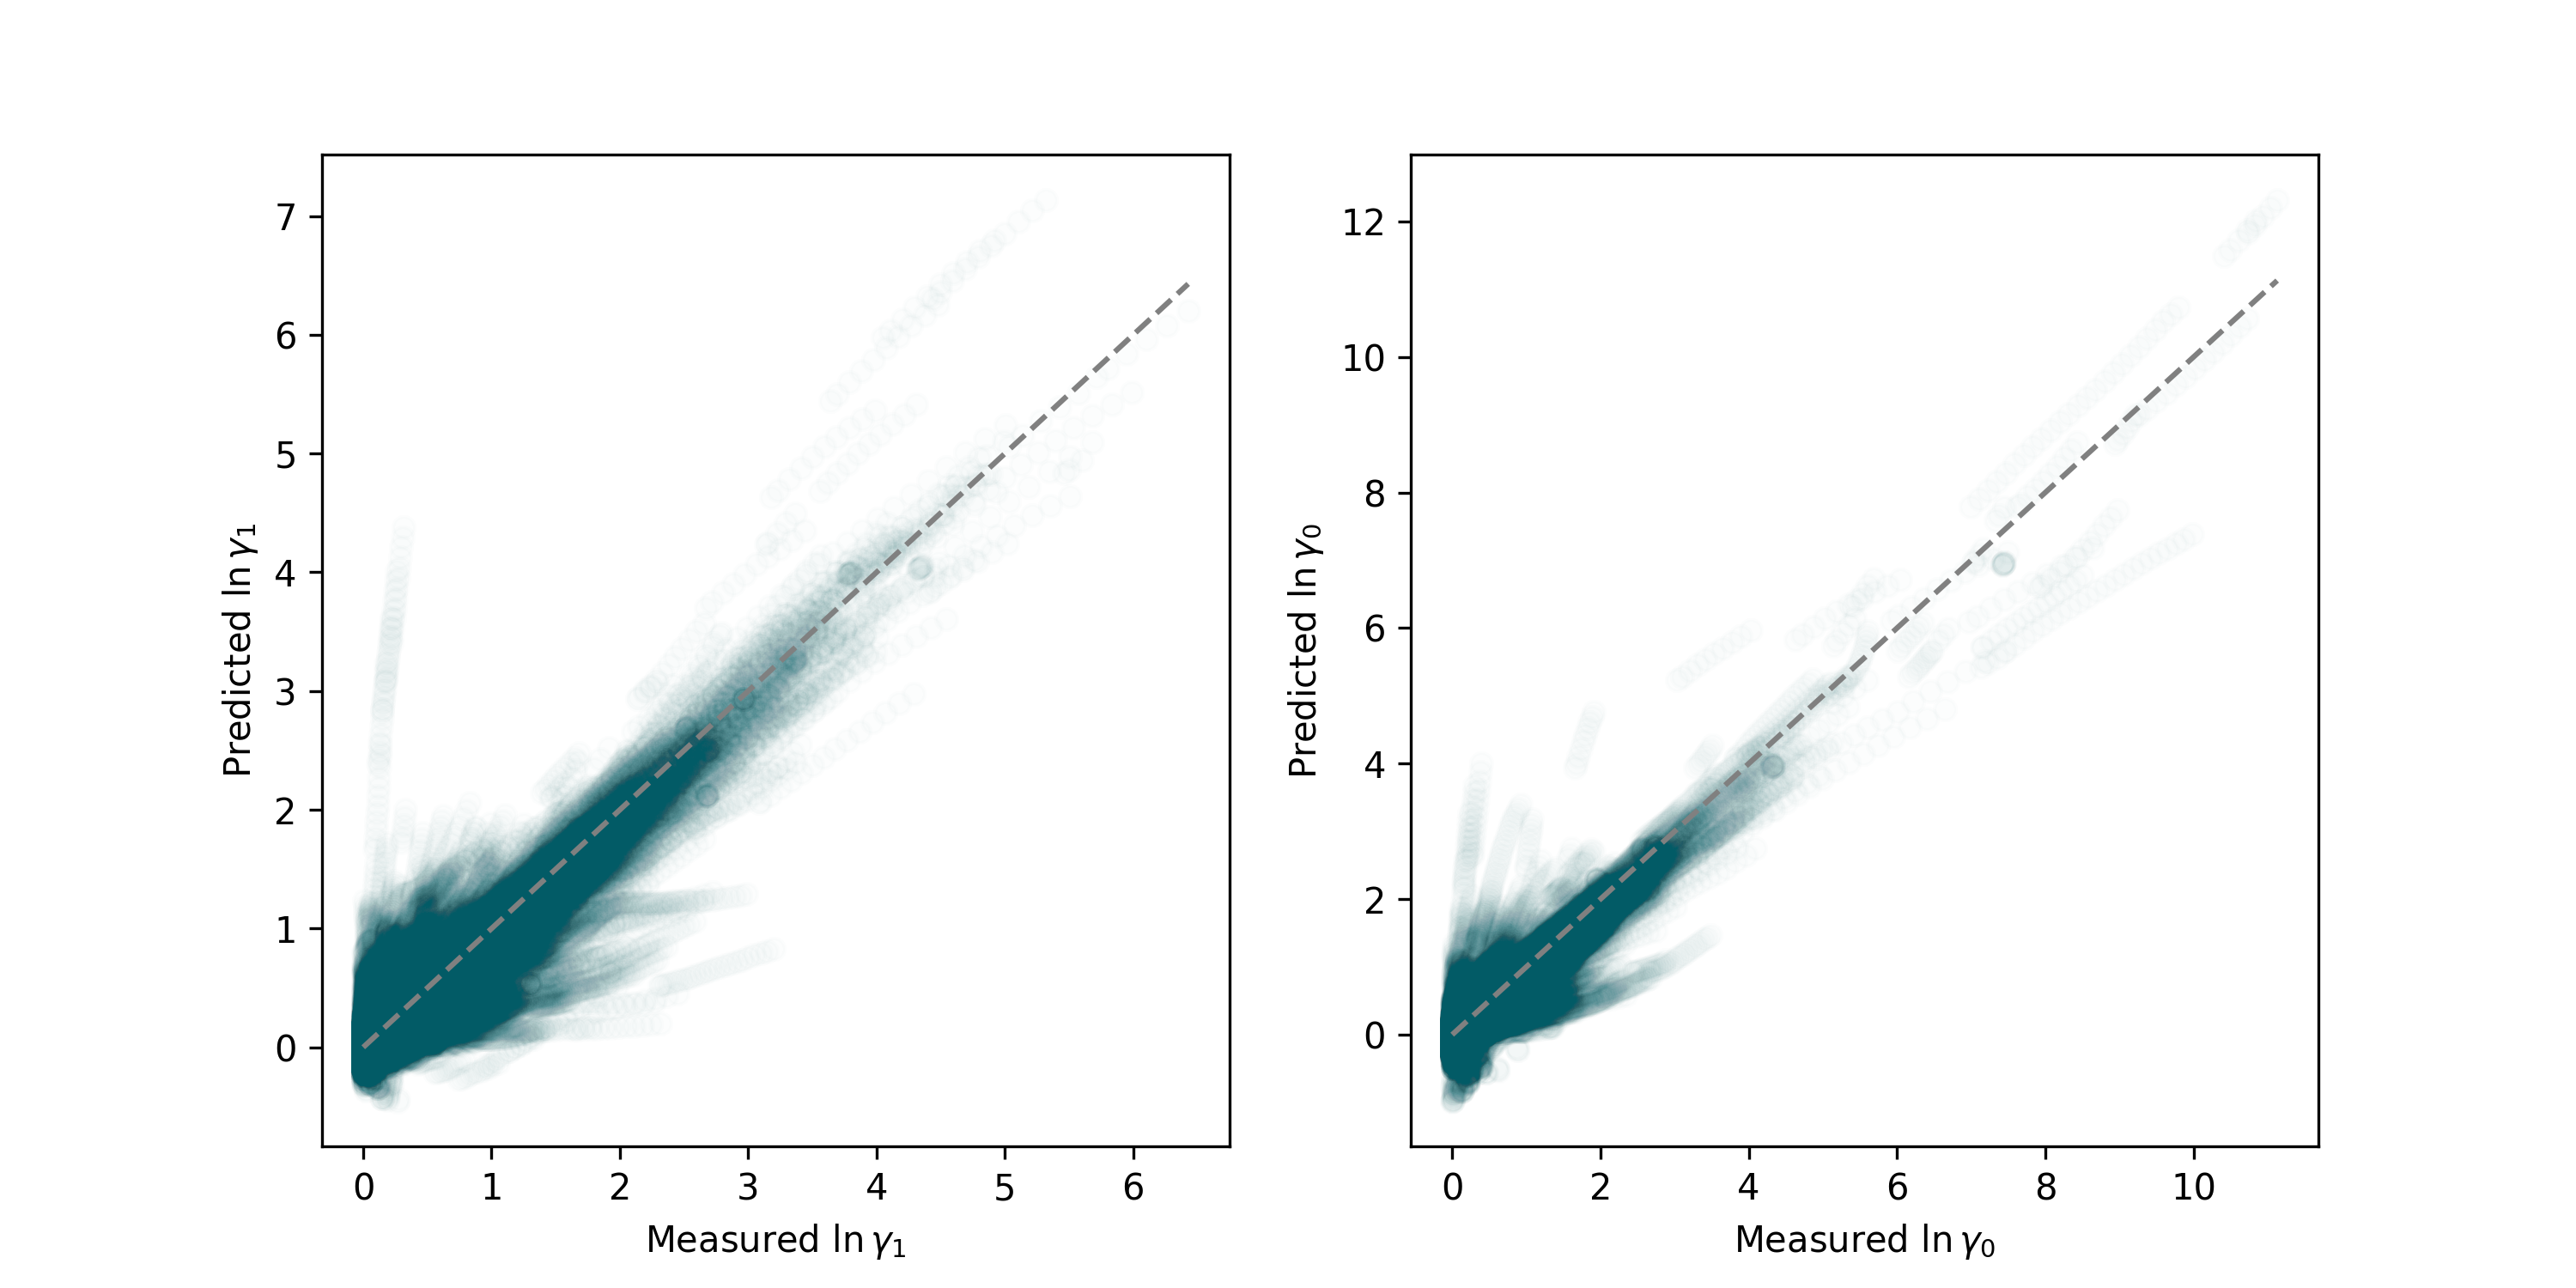
\includegraphics[width=\textwidth]{gfx/Chapter06/cosmo_base_test_indp_parity_plot.png}
    \caption{Caption}
    \label{fig:my_label}
\end{figure}


\section{Challenges with DeepGamma}

While \textit{DeepGamma}, can offer 1900x speed-up compared to the original quantum simulations, it has several limitiations. First, it relies solely on quantum simulation data, which are themselves not fully predictive of experimental results. Second, the results are not necessarily thermodynamically consistent. This is due to the feedforward network used in the readout phase not being permutation invariant; the activity coefficient predictions are not independent of the order of the molecules. Finally, the model does not scale past binary mixtures. Therefore, I looked to develop a more comprehensive approach to thermodynamic predictions using deep learning.

% *****************************************
% *****************************************
% *****************************************
% *****************************************
% *****************************************
